\chapter{Grundlagen neuronaler Netze}
\label{kapitel_neuralnetworks}

In diesem Abschnitt werden Künstliche Neuronale Netze\cite{dayhoff1990neural}, kurz KNN, als Forschungsgegenstand der Informatik eingeführt und deren mathematischen Grundlagen präzisiert. 
Sie stellen informationsverarbeitende Systeme nach dem Vorbild von tierischen beziehungsweise menschlichen Gehirnen dar und bestehen aus Neuronen in gewissen Zuständen und Schichten, die über gewichtete Verbindungen miteinander gekoppelt sind. Jene Gewichte sind als freie Parameter des neuronalen Netzes zu verstehen und können während des Trainingsprozesses so angepasst werden, um eine entsprechende Aufgabe zu lösen.  
Gelingt dies, so können neuronale Netze genutzt werden, um bestimmte Muster in Daten, typischerweise in Bildern, Audio oder Stromdaten, effizient zu erkennen\cite{pandya1995pattern, pao1989adaptive, urbaniak2021quality}.
Sie eignen sich daher für viele typischen Aufgaben des maschinellen Lernens, beispielsweise für die Klassifikation digitalisierter Objekte.

Im ersten Abschnitt wird das Perzeptron\cite{rosenblatt1958perceptron} als Grundeinheit eines neuronalen Netztes eingeführt. 
Im folgendem Abschnitt wird das Konzept der Multi-Layer-Perzeptronen\cite{werbos1988generalization} durch die Kopplung mehrerer Perzeptronen mit bestimmten Übertragungs- und Aktivierungsfunktion in einem Netz erläutert. Diese Repräsentierung eines KNN wird im weiteren Verlauf dieser Arbeit genutzt. 

\section{Das Perzeptron}
\label{perzeptron_abs}
Zunächst wird das \textit{Perzeptron} ähnlich wie in Minsky \cite{minsky2017perceptrons} als fundamentaler Baustein eines neuronalen Netzes eingeführt. Das Perzeptron stellt im Allgemeinen ein erstes trainierbares Modell dar und wird oft als Basis moderner KNN angeführt. 
\begin{defi}[Perzeptron]
    \label{def_neuron}
    Für eine gegebene Funktion $\psi: \RR \rightarrow \RR$, einen Vektor $w \in \Rnv$ und ein Skalar $\theta \in \RR$ wird die Funktion 
    \[ \
    \Psi: \RR^n \rightarrow \RR, \; \; \; x \mapsto \psi(w^T x +\theta)=:y,
    \]
    \textit{Perzeptron} genannt. Mit $x \in \Rnv$ wird die vektorwertige Eingabe und mit $y \in \RR$ die skalare Ausgabe des Perzeptrons bezeichnet. Dabei ist mit $w^Tx=\sum_{i=1}^n w_i x_i$ das Standardskalarprodukt im euklidischen Vektorraum $\Rnv$ gemeint. Die Komponenten von $w$ werden Gewichte und der Skalar $\theta$ Schwellwert oder auch Bias genannt.
\end{defi}
Die Funktionsweise eines Perzeptrons ist in Abbildung \ref{funktionsweise_neuron} dargestellt.

\begin{figure}[h]
    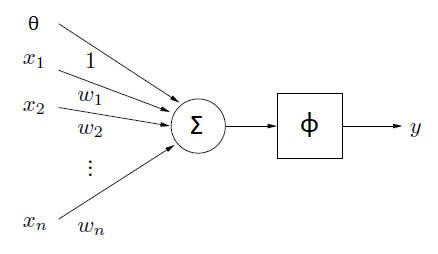
\includegraphics[width=0.8\textwidth]{pics/chapter_neuralnetworks/perzeptron.png}
    \centering
    \caption{Arbeitsweise eines Perzeptrons mit entsprechender Notation aus Definition \ref{def_neuron}.}
    \label{funktionsweise_neuron}
\end{figure}

Bei der Wahl der Funktion $\psi$ gibt es mehrere Möglichkeiten. Wird wie in Minsky\cite{minsky2017perceptrons} die Heavyside-Funktion
\begin{equation*}
    \psi: \RR \rightarrow \RR, \; \; \;
    \psi(x)=\begin{cases}
       1 &, x \geq 0 \\
       0 &, \text{sonst}
    \end{cases}
\end{equation*} 
genutzt, kann das Perzeptron als binärer Klassifikator wie in \ref{abs_linear_trenn} interpretiert werden. Dabei dient $w^Tx+\theta=0$ als trennende Hyperebene. Ist $w^Tx+\theta<0$, so ist $\psi(x)=0$ und $x$ wird der Klasse $K_{-1}$ zugeordnet. Gilt jedoch $w^Tx+\theta \geq 0$ und damit $\psi(x)=1$, so ist der Vektor $x$ der Klasse $K_1$ zugehörig. 

Für ein Klassifikationsproblem, bei dem die Klassen nicht linear trennbar sind, scheitern diese einfachen Perzeptronen. Hier wird oft das zweidimensionale XOR-Problem angeführt, bei denen die Punktmengen $P_{-1}=\{(0,0),(1,1)\}$ und $P_{1}=\{(1,0),(0,1)\}$ getrennt werden sollen. Um solche Aufgaben zu lösen, ist es notwendig, mehrere Perzeptronen geschickt zu verknüpfen, um komplexe Entscheidungsgrenzen zu erhalten.

\section{Multi-Layer-Perzeptron}
\label{MLP_abs}
In dieser Arbeit wird ein Künstliches Neuronales Netz als eine Menge von Perzeptronen, die in gewissen Schichten partitioniert und miteinander verbunden sind, notiert. Diese sogenannten \textit{Multi-Layer-Perzeptronen}, kurz MLP,  gelten als erste tiefe neuronale Netze und sind seit den späten 1980er Gegenstand der Forschung\cite{bourlard1990links,bounds1988multilayer,MLPbook}. Zunächst sind einige Definition notwendig, um eine lesbare Notation von MLPs zu geben.

\begin{defi}[Übertragungsfunktion]
    \label{def_net}
    Für eine gegebene Matrix $W \in \RR^{n \times m}$ und einen Vektor $b \in \RR^m$ ist 
    \[ 
    \Psi^{W,b}: \RR^n \rightarrow \RR^m, \; \; \; x \mapsto W^T x +b
    \]
    als Übertragungsfunktion definiert. Der Vektor $y=\Psi^{W,b}(x) \in \RR^m $ wird als Netzeingabe bezeichnet.
\end{defi}
Hierbei ist $W$ eine Gewichtsmatrix und $b$ ein Biasvektor, welche als freie Parameter fungieren und die Netzeingabe eines Eingabevektors $x \in \RR^n$ auf lineare Art und Weise beeinflussen. Um auch nichtlineare Zusammenhänge darzustellen, werden Aktivierungsfunktionen benutzt.

\begin{defi}[Aktivierungsfunktion]
    \label{def_act_f}
    Eine stetige, monoton steigende und nicht notwendigerweise lineare Funktion $\psi: \RR \rightarrow \RR$ wird als Aktivierungsfunktion bezeichnet.
\end{defi}
Es sei erwähnt, dass auch nicht monotone Aktivierungsfunktionen genutzt werden können, beispielsweise radiale Basisfunktionen\cite{radialbasis}, welche jedoch in dieser Arbeit nicht weiter von Interesse sind.
Typische Aktivierungsfunktionen, die heutzutage verwendet werden, sind die:
\begin{align*}
    \text{Identität}: \; \;\psi(x)&=x, \\
    \text{Logistische Funktion}: \; \;\psi(x)&=\frac{1}{1+\mathrm{e}^{-x}}, \\
    \text{Tangens Hyperbolicus}: \; \;\psi(x)&=\tanh(x), \\
    \text{ReLU (rectified linear unit)}: \; \;\psi(x)&=\max\{0,x\}.
\end{align*}

\begin{bem}
    Ist $\psi$ eine Aktivierungsfunktion, so wird für $x \in \RR^n$ mit 
    \[\psi(x):=\left(\psi(x_1), \ldots, \psi(x_n)\right)^T \in \RR^n
    \]
    der Vektor bezeichnet, welcher sich durch die elementweise Auswertung der Aktivierungsfunktion $\psi$ an den Stellen $x_1, \ldots, x_n$ ergibt. 
\end{bem}

Bei Klassifikationsproblemen wird oft die \textit{Softmax}-Funktion\cite{denker1990transforming} genutzt, welche die gesamte Eingabe berücksichtigt. Im Abschnitt \ref{task_training} wird erläutert, warum sich in diesem Fall diese Softmax-Funktion anbietet.

\begin{defi}[Softmax]
    Für $x \in \RR^n$ wird die Funktion $\psi: \RR^n \rightarrow (0,1]^n$ mit 
    \[
        \psi(x):=\left(\frac{\mathrm{e}^{x_1}}{\sum_{i=1}^n \mathrm{e}^{x_i}}, \ldots,\frac{\mathrm{e}^{x_n}}{\sum_{i=1}^n \mathrm{e}^{x_i}} \right)^T
    \]
    als Softmax-Funktion definiert. Da sich die Einträge des Vektors $\psi(x)$ zu Eins summieren, kann die Aktivierung als eine Verteilung interpretiert werden, welche die Wahrscheinlichkeiten für bestimmte Klassenzugehörigkeiten angeben.  
\end{defi}

Für den späteren Trainingsprozess ist es nützlich, die Ableitung der verwendeten Aktivierungsfunktion, sofern sie exisitiert, zur Verfügung zu haben. Zudem ist es möglich, für bestimmte Aktivierungsfunktionen die Ableitung nur mithilfe der verwendeten Funktion zu berechnen.

\begin{lem}
    \begin{itemize}
        \item[(i)] Für die ReLU $\psi(x)=\max\{0,x\}$ gilt
         \[\psi'(x)=\begin{cases}
            0 &, x <0 \\
            1 &, x >0
        \end{cases}. 
        \]
        An der Stelle 0 ist die Ableitung nicht definiert und wird oft mit $\psi'(0)=\frac{1}{2}$ festgelegt.
        \item[(ii)] Für die logistische Funktion $\psi(x)=\frac{1}{1+\mathrm{e}^{-x}}$ gilt
        \[ 
            \psi'(x)=\psi(x)(1-\psi(x)) 
        \]
        für alle $x \in \RR$.
        \item[(iii)] Für den Tangens Hyperbolicus $\psi(x)=\tanh(x)$ gilt
        \[ 
            \psi'(x)=1-\psi^2(x) 
        \]
        für alle $x \in \RR$.
    \end{itemize}
\end{lem}


Ähnlich der Definition des Perzeptron \ref{def_neuron} wird nun eine Schicht als Verknüpfung von Übertragungsfunktion und Aktivierungsfunktion definiert.

\begin{defi}[Neuronenschicht]
    Ist $\Psi^{W,b}$ eine Übertragungsfunktion mit den Parametern $W \in \RR^{n \times m}, b \in \RR^m$ und $\psi$ eine Aktivierungsfunktion, so wird das Paar $(\Psi^{W,b}, \psi)$ als Schicht $\mathcal{S}$ bezeichnet. Für eine Eingabe $x \in \RR^n$ ist die Ausgabe $y \in \RR^m$ der Schicht $\mathcal{S}$ durch
    \[y=\psi \circ \Psi^{W,b}(x)= \psi\left(\Psi^{W,b}(x)\right)
        \] 
        gegeben. Die Komponenten $y_i$ werden für $1 \leq i \leq m$ Neuronen der Schicht $\mathcal{S}$ genannt und gleichen jeweils der Ausgabe eines einfachen Perzeptrons wie in Definition \ref{def_neuron}. Eine Schicht besteht aus $m$ Perzeptronen $\tilde{\Psi}_i$ mit $y_i=\tilde{\Psi}(x_i)=\psi(W_{i,:}^T x+b_i)$ für $1 \leq i \leq m$.
\end{defi}
Im Hinblick auf MLPs werden nun mehrere Schichten so verbunden, dass die Ausgabe einer Schicht $\mathcal{S}_k$ als Eingabe einer darüberliegenden Schicht $\mathcal{S}_{k+1}$ für ein $k \in \mathbb{N}$ dient. Die Anzahl der Neuronen kann dabei von Schicht zu Schicht variieren. Dementsprechend werden die Dimensionen der beteiligten Gewichtsmatrizen $W^{(k)}$ und Biasvektoren $b^{(k)}$ passend gewählt. 
Um die Notation übersichtlich zu halten, bezeichne $\Psi^{W^{(k)},b^{(k)},\psi_{k}}$ die Schicht $\mathcal{S}_k$ mit $\Psi^{W^{(k)},b^{(k)},\psi_{k}}(x):= \psi_{k} \left(\Psi^{W^{(k)},b^{(k)}}(x)\right)$.

\begin{defi}[Multi-Layer-Perzeptron, vgl. gruening]
    Für eine gegebene Anzahl $l \in \mathbb{N}, \; l>1$ von Schichten $\Psi^{W^{(1)},b^{(1)},\psi_{1}}, \ldots, \Psi^{W^{(l)},b^{(l)},\psi_{l}}$ bezeichne $s_l \in \mathbb{N}$ die Anzahl der Neuronen in Schicht $l$. Für eine Eingabe $x \in \RR^{s_0}$ lässt sich die Ausgabe $y \in \RR^{s_l}$ eines Multi-Layer-Perzeptron  $\Lambda_l: \RR^{s_0} \rightarrow \RR^{s_l}, \; x \mapsto y$ mit $l$ Schichten durch
    \[
        y=\Psi^{W^{(l)},b^{(l)},\psi_{l}} \circ \ldots \circ \Psi^{W^{(1)},b^{(1)},\psi_{1}}(x)
    \]
    berechnen. Dabei gelten für die Gewichtsmatrizen die Dimensionsbedingungen
    \[{}_1W^{(1)}=s_0, \; \; {}_2W^{(l)}=s_l, \; \; \forall i \in [l-1]: \; {}_2W^{(i)}={}_1W^{(i+1)}.
        \] 
    Die Eingabeschicht $\mathcal{S}_0$ besitzt keine Parameter $W$ und $b$ und besteht nur aus dem Eingabevektor $x \in \RR^{s_0}$. Die letzte Schicht $\Psi^{W^{(l)},b^{(l)},\psi_{l}}$ wird als Ausgabeschicht bezeichnet. Weiter werden die Schichten $\mathcal{S}_1, \ldots, \mathcal{S}_{l-1}$ als verdeckte Schichten definiert. Die Funktionsauswertung $\Lambda_l(x)$ für eine Eingabe $x$ wird Vorwärtsrechnung, engl. \textit{forward propagation}, genannt.
\end{defi}
Das MLP-Modell wird im weiteren Verlauf dieser Arbeit repräsentativ als Künstliches Neuronales Netz bezeichnet. Das zuvor angesprochene XOR-Problem kann nun beispielsweise mithilfe eines KNN bestehend aus zwei Schichten gelöst werden\cite{Goodfellow-et-al-2016}.
Es lassen sich zwischen Modell- und Hyperparameter von KNNs unterscheiden.

\begin{defi}[Hyper- und Modellparameter]
    Sei für $l \in \mathbb{N}$ ein KNN $\Lambda_l$ gegeben. Dann werden die Eingabe- und Ausgabedimension $s_0, s_l$, die Anzahl $l$ der Schichten, die Anzahl $l-1$ der verdeckten Schichten sowie die verwendeten Aktivierungsfunktion $\psi_l$ Hyperparameter des neuronalen Netzes genannt.
    Die Gewichtsmatrizen und Biasvektoren mit den entsprechend passenden Abmessungen stellen die Modellparameter $\mathcal{W}:=\{(W^{(i)},b^{(i)}): \; i=1, \ldots, l\}$ des neuronales Netzes dar. 
\end{defi}
Die Hyperparameter werden oft anwendungsspezifisch für das jeweilige Problem gewählt, während die Modellparameter dynamisch in einem Trainingsprozes angepasst werden, sodass die gegebene Aufgabe zufriedenstellend gelöst wird. Wie sies geschieht, wird im folgenden Abschnitt \ref{task_training} erläutert.

\section{Training neuronaler Netze}
\label{task_training}
Künstliche Neuronale Netze gehören zu den typischen Vertretern von maschinellen Lernalgorithmen, welche hinsichtlich einer bestimmten Aufgabe, engl. \textit{task T}, und einem Leistungsmaß, engl. \textit{perfomance P} an der Erfahrung, engl. \textit{experience E} lernen\cite{Goodfellow-et-al-2016}. Dabei ist mit Lernen gemeint, dass das Computerprogramm bezüglich der Aufgabe $T$ sein Leistungsmaß $P$ mit wachsener Erfahrung $E$ schrittweise steigert. Wie in Kapitel \ref{fund} erläutert, gibt es viele verschiedene Aufgaben, wie die Regression, Klassifikation oder Clusterung bestimmter Objekte. 

In den folgenden Abschnitten wird das Klassifikationsproblem im Mittelpunkt stehen. Weiter werden KNNs als Modellschätzer aus der Wahrscheinlichkeitstheorie interpretiert und fundamentale Aussagen wie das \textit{Universal-Approximation-Theroem}\cite{HORNIK1989359} gegeben. Schließlich wird bezüglich der Klassifikationsaufgabe das Training neuronaler Netze erläutert.

\begin{defi}
    Sei die Mengen $D \subset \RR^n$ und $\mathcal{C}=\{c_1, \ldots, c_m\}$ gegeben. Eine Funktion $f: D \rightarrow \mathcal{C}$, welche ein Element aus $D$ einer Klasse $c_i \in \mathcal{C}$ zugeordnet, wird Klassifikationsfunktion genannt. Hier gibt es $m \in \mathbb{N}$ verschiednen Klassenlabels.
\end{defi}

Das Ziel beim Klassifikationsproblem ist die Approximation einer bestimmten Klassifikationsfunktion durch eine Modell $\tilde{f}: D \rightarrow \mathcal{C}$. In dieser Arbeit werden dafür KNNs genutzt, welche als probabilistische Modelle auf folgende Weise genutzt werden. Auf der Ergebnismenge $\Omega= D \times \mathcal{C}$ sei die nicht bekannte gemeinsame (Wahrscheinlichkeits-) Verteilung $p_{D}(x,c)$, genannt Datenverteilung, gegeben. Ein Modell soll nun so konstruiert werden, das die posterior-Verteilung $p_D(\cdot \; | \; x)$ der Klassen  geschätzt wird. In dieser Arbeit werden KNNs so benutzt, dass die Klassenzugehörigkeit direkt anhand der Eingabe $x \in D$ geschätzt wird. Die Funktion $P_D: D \rightarrow [0,1]^m$ mit
\begin{equation}
    P_D(x):=\left(p_D(c_1 \; | \; x), \ldots, p_D(c_m \; | \; x)\right)^T \in \RR^m
\end{equation} soll für alle $x \in D$ approximiert werden. Dazu wird die Approximation $P_{Modell}: D \rightarrow [0,1]^m$ mit 
\begin{equation}
    P_{Modell}(x;\mathcal{W}):=\left(p_{Modell}(c_1 \; | \; x; \mathcal{W}), \ldots, p_{Modell}(c_m \; | \; x; \mathcal{W})\right)
\end{equation}
 für alle $x \in D$ genutzt, welche von den Modellparametern $\mathcal{W}$ abhängig ist. Das abgeleitete Modell ist die Klassifikationsfunktion
\begin{equation}
    f_{Modell}(x):= \underset{c \in \mathcal{C}}{\mathrm{argmax}} \; p_{Modell}(c \; | \; x)
\end{equation}

Es stellt sich die Frage, in wie fern das MLP als Modell genutzt werden kann, um beliebige Datenverteilungen $P_D$ zu approximieren. Folgender Satz liefert dazu die Antwort.

\begin{satz}[Universal-Approximation-Theroem]
    
\end{satz}